\chapter{\sc Graphene}
\label{ch:Graphene}

\section{Carbon and its Allotropes}

Carbon is possibly the most ubiquitous atomic element known to man. The fourth most abundant element in the entire universe behind only hydrogen, helium, and oxygen, carbon is found essentially everywhere one looks for it in one form or another. Originating from stellar nucleosynthesis, carbon is an important element in the evolution of different chemical elements in the history of the universe \cite{katsnelson}. As a result of its abundance, carbon plays a special role in human history with frequent and diverse usage in everything from metallurgy to medicine, and art to energy.

\begin{equation}
  \label{eq:photosynthesis}
  \ce{6 CO2(g) + 6 H2O(l) ->[ \gamma ] C6H12O6(s) + 6 O2(g)}
\end{equation}

Carbon has atomic number six and a valence number of four corresponding to an electron configuration of  $1s^2 2s^2 2p^2$. The tetravalent aspect makes carbon unique due the vast number of bonding schemes allowed by this electron configuration. The large number of bond formations allows an endless variety of molecules and allotropes based on carbon to form readily. Simple gases such as \ce{CO_2} and \ce{CH_4} are common to everyday life, however, more complex molecules like glucose, \ce{C_{6}H_{12}O_6}, are crucial to all life as we know it at the cellular level both in the Krebs cycle and also in photosynthesis. In fact, carbon is denoted the \emph{material prima}, or fundamental substance, for all life \cite{geim-elec}. The importance of carbon to the photosynthetic cycle is shown in equation \ref{eq:photosynthesis}. The complex sugars and hydrocarbon chains represent of the wide array of organic compounds possible through carbon chemistry, however, there are many forms of molecules and materials that can be made purely from carbon and no other elements.

The word allotrope refers to distinct physical forms of material made from a single element; carbon has numerous stable allotropes. The wide variety of carbon allotropes expose the rich geometry afforded to different bonding schemes from simple rings and linear chains to complex three-dimensional structures. Carbon is the only element thus far found to be stable in materials ranging from zero to three dimensions. This has profound implications on the material properties carbon can adopt, as a material's dimensionality is one of its most defining properties \cite{novoselov-2d}. Fullerene molecules made of nearly spherical cages of carbon rings demonstrate carbon in zero-dimensional form, though they are sometimes referred to as quasi-zero-dimensional. Carbon nanotubes are the manifestation of carbon in one-dimensional objects, and can be viewed as the linear extension of a buckyball in one direction. Graphene, a planar carbon structure, extends carbon to two-dimensional materials, and has the same structure as an unzipped or unrolled carbon nanotube. Finally graphite and diamond represent two separate ways of carbon bonding in three dimensions. These variants of solid carbon all have distinctly different physiochemical properties.

Graphite, named after the Greek \emph{graphos}, meaning to write, consists of many layers of $sp^2$ bonded carbon; each layer can be considered an individual graphene sheet \cite{history-thermodynamics}. These layers are only weakly bonded to each other in the direction perpendicular to the basal plane through van der Waals forces. This bond configuration is very weak relative to the covalent in-plane bonds and as a result the inter-layer coupling in graphite is also weak which allows the layers to slide against one another with relative ease. As a result, graphite is an ideal material for use in pencils or other marking devices and as a lubricant.

The primary material of interest in this thesis is the individual graphite layers known as graphene. The two-dimensional nature of this material directly bestows many interesting physiochemical properties. As the first direct evidence that two-dimensional materials can be thermodynamically stable, the discovery of graphene has spawned an entire new field of material science and physical research.

\section{Carbon in Two Dimensions: Graphene}
  \subsection{Discovery and History}
Discovery and usage of graphite dates back over 500 years \cite{honeycombcarbon}. The original uses for graphite were for writing, marking, and art, however, in the present graphite sees use as an industrial lubricant as well as the primary moderator in nuclear fission reactors. The structure and properties of graphene have been studied from a theoretical standpoint since the early work by Wallace in 1947 \cite{wallace}. This early work laid the foundation of considering graphite as a collection of weakly interacting carbon layers. In this sense, each carbon layer can be effectively considered independent from the others and thus the electronic structure can be modeled by considering only one layer. At the time, however, it was widely believed that a single layer by itself would be thermodynamically unstable \cite{Geim}.

	The study of epitaxial growth of carbon layers on various metal surfaces dates back to the 1970's. Measurements of the properties of the carbon layers were, however, always skewed by the strong interaction between carbon and metals. This made measuring pure graphene-like properties difficult. In the early 2000's work continued on isolating single or few carbon layers from graphite. Graphite is commonly used in STM laboratories as an ideal sample for calibration of the microscope due to the periodic surface structure and ease of sample preparation. A common method to prepare the surface of graphite is simply to apply adhesive tape to the surface and peel away the tape. This adhesion between surface carbon layers and the tape is much stronger than the layer-layer bonding in the graphite. Thus, carbon layers can easily be peeled away from a bulk graphite crystal.

	The breakthrough in isolating single layer graphene came from Andre Geim and Kostya Novoselov at the University of Manchester in 2004. Careful analysis of the carbon remnants on adhesive tape from cleaved graphite lead to the discovery that some exfoliated carbon layers were thicker than others. Continued work lead to the isolation of single layer carbon after an important discovery that graphene would be optically visible when placed on a silicon dioxide substrate with carefully chosen thickness \cite{Geim}. Confirmation of single layer graphene demonstrated for the first time that a material could be stable as a single atomic layer. This work, which lead to a Nobel prize for Geim and Novoselov in 2010, spawned an explosion in fundamental research of the properties of two-dimensional materials.

  \subsection{Structure}
 Graphene consists solely of $sp^2$ hybridized carbon atoms. This bond configuration is found in single graphene sheets, in three-dimensional graphite, as well as in other organic molecules such as benzene. The structural bonds connecting nearest neighbor carbon atoms are called $\sigma$ bonds. In the $sp^2$ configuration each carbon atom is bonded covalently to three other carbon atoms with an average bond distance of 1.42 {\AA}. Mathematically the $\sigma$ bond in graphene is a linear combination of the $2s$ and $2p$ electron orbitals. In order to minimize the overlap between individual $\sigma$ bonds, the bonds are separated by an angle of $120^{\circ}$. All three bonds lie within a single two-dimensional plane and thus accordingly, graphene is deemed a two-dimensional material.

 \begin{figure}
    \centering
         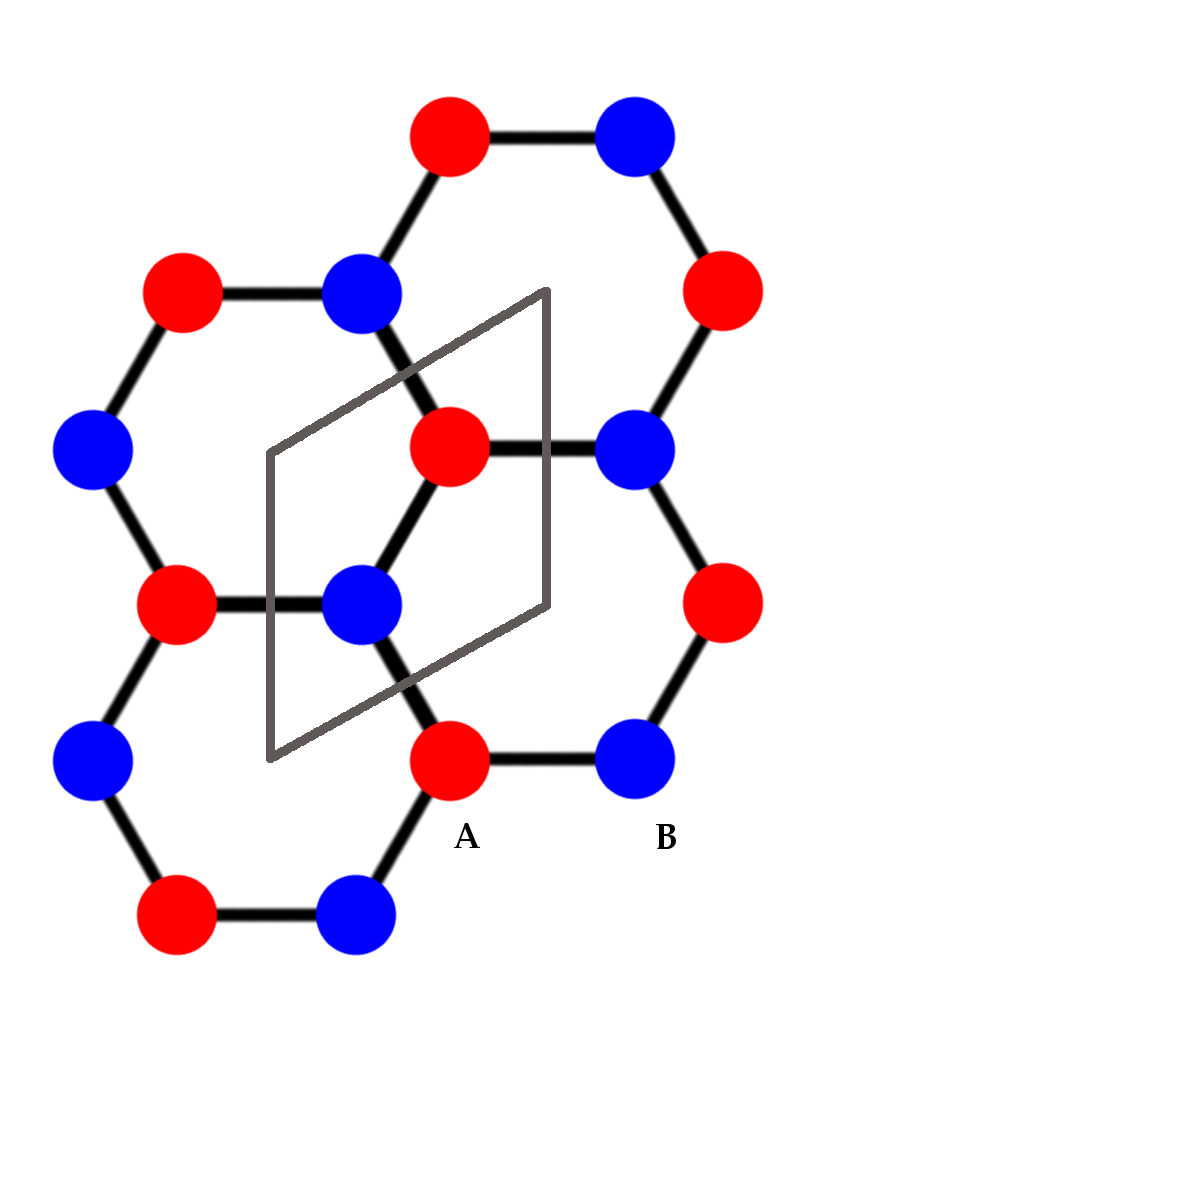
\includegraphics[scale=0.65]{figs/graphene-unit-cell.png}
    \caption{
Graphene honeycomb lattice shown composed of alternating A (red) and B (blue) carbon atoms. The graphene unit cell is highlighted in grey showing that the cell contains two distinct carbon atoms.
}
    \label{fig:graphene}
\end{figure}


 \begin{figure}
     \centering
         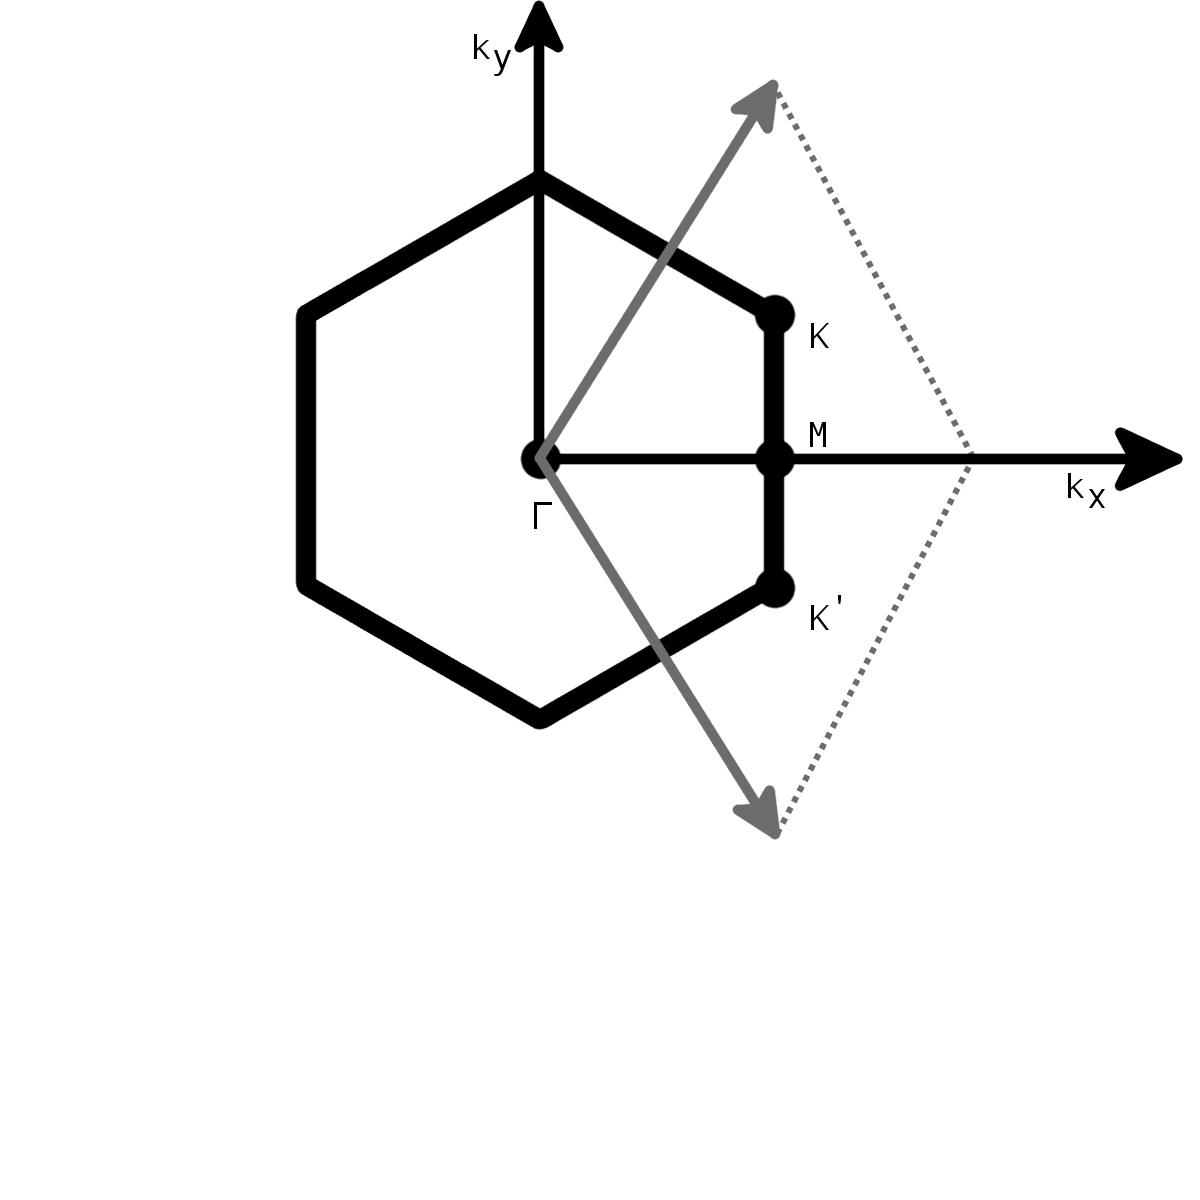
\includegraphics[scale=0.55]{figs/graphene-reciprocal-lattice.png}
     \caption{ The graphene real space hexagonal lattice is accompanied by a hexagonal reciprocal space lattice. Shown here is the reciprocal unit cell relative to the first Brillouin zone; the important high symmetry points are labeled, notably the K and K' points are distinct from one another.
}
     \label{fig:graphene-reciprocal}
\end{figure}

 Carbon is tetravalent, thus, outside of the structural bond configuration, which occupies three of the four valence electrons, each carbon atom in the graphene structure has one free electron. Again to minimize the overlap with the structural bonding $\sigma$ orbitals, the free electron fills the remaining $n=2$ electron orbital. Conventionally the electron orbitals that hybridize to create the $\sigma$ bonds are labeled as the spherically symmetric $2s$ orbital as well as the $2p_x$ and $2p_y$ planar orbitals. The graphene structure then lies solely in the x-y Cartesian plane. The sole unfilled $n=2$ orbital is then the $2p_z$ orbital, which lies perpendicular to the structural bonding plane. For each carbon atom, one electron fills the $2p_z$ orbital and is not responsible for in-plane structure. The nearest neighbor carbon distance is large enough that there is very weak overlap between the $2p_z$ orbitals. However, there is still a non-zero overlap between neighboring $2p_z$ orbitals, this electron orbital overlap is called a $\pi$ bond.

 The out of plane $\pi$ bonds in an individual graphene sheet are responsible for the three dimensional structure of graphite when multiple layers are stacked atop one another. The $\pi-\pi$ stacking between layers is very weak relative to the intra-planar $\sigma$ bonding. This weak bonding allows individual graphene planes to slide parallel to the basal plane relative to other carbon layers with ease. Considering just a single graphene layer, the pi bonds are delocalized from the planar structure, and thus the electrons in these orbitals are responsible for the unique electronic properties of graphene, which will be explored later.

 Since the structural bonding in graphene lies within a two-dimensional plane, graphene is labeled as a two-dimensional material. Currently graphene is the thinnest material in existence that is thermodynamically stable at ambient conditions and has been prepared in a lab setting. While there are other single element two-dimensional materials, given the general trend for average atomic radii there are few options for materials that would be thinner than graphene. In fact, many other group IV elements such as silicon, germanium and tin have been theorized to have two-dimensional allotropes. They are named in similar fashion to graphene, namely silicene (Si), germanene (Ge), and stanene (Sn). While the carbon atoms in graphene remain coplanar, the hexagonal arrangement of atoms in other group IV two-dimensional materials generally adopts a buckled bilayer structure.

Here it is worth noting that while the theoretical structure of freestanding graphene should be atomically flat up to micrometer scales, there are currently no methods of producing large scale freestanding graphene, thus in practice the structure of the carbon layer will be dependent on the substrate on which it lies. Graphene can be grown atop a wide variety of crystalline and amorphous substrates from simple metals such as nickel and copper to more complex semiconductor surfaces such as silicon carbide. The structure of the carbon layer can change drastically as a result of the topology of the underlying substrate surface structure and thus as a result the properties of the graphene layer may depart from those of ideal freestanding graphene.

  \subsection{Significance: Paradigm shift to 2D}

 While it has already been mentioned that the discovery of graphene essentially launched the field of two-dimensional materials into notoriety, the significance warrants further discussion. After the isolation of graphene, numerous other layered van der Waals materials were examined as candidates for two-dimensional isolation. Quite quickly it was found that materials such as hexagonal boron nitride, molybdenum disulfide, and niobium diselenide could be treated in a similar manner to graphite to produce two-dimensional materials \cite{novoselov-2d}. The later materials fall into a category of materials called transition metal dichalcogenides, TMDs. It is now known that this family of materials hosts a plethora of materials suited for two-dimensional applications. These further studies demonstrate that graphene is not the anomaly in the nouveau two-dimensional material world; rather there exists a potentially endless realm of new materials with distinct and exciting properties.

  The discovery of materials that can be isolated in two-dimensional form, while noteworthy as it was originally theorized to be impossible, only provides the scaffolding for the search for new physics in two-dimensions. The study of material properties in the two-dimensional limit truly garners excitement in the world of material science. The vast assortment of two-dimensional materials fully spans the configuration space of material properties. While graphene possesses unique electronic properties as a zero-gap semiconductor, some TMDs display interesting changes in their band structure as their thickness decreases to the two-dimensional limit. For example, bulk molybdenum disulfide, \ce{MoS_2}, is an indirect gap semiconductor with a band gap of approximately $1.23$ eV. When the bulk crystal is exfoliated to produce two-dimensional monolayer samples, the electronic properties change drastically and the material manifests as a direct gap semiconductor with a band gap of roughly $1.8$ eV \cite{monolayer-mos2, 2d-atlas}. While many TMDs are characterized as semiconducting materials, other 2D materials exhibit more exotic electronic properties such as superconductivity and charge density waves \cite{2D-TMDs}.

  That many two-dimensional materials are stable in ambient conditions while also retaining their unique properties is of great significance. The variety of electronic properties found in two-dimensional materials makes them ideal for applications in new ultra-thin flexible electronic devices. The optical properties found in two-dimensional materials open new avenues for photovoltaic devices as well as photosensors for light spectra difficult to absorb with conventional silicon technology \cite{ graphene-2d-optoelectronics}. Furthermore, there are many novel electronic devices, such as tunnel-junction transistors, which are only functional when constructed with ultra-thin heterojunctions. Two-dimensional semiconductors provide a new avenue for exploration of these devices. Many interesting properties of two-dimensional materials stem directly from the unique surface structure adopted by the materials; the link between graphene's structure and its sought after characteristics will be explored further.

\section{Properties and Applications}
  \subsection{Structure Review}
Graphene forms a two-dimensional honeycomb lattice with a nearest neighbor separation of 1.42 {\AA} and a lattice constant of 2.46 {\AA}. The graphene unit cell contains two distinct carbon atoms, thus the graphene lattice can be considered two interpenetrating trigonal sublattices. These sublattices are commonly referred to as A and B as shown in figure \ref{fig:graphene}. This lattice geometry, where A atoms are bonded to only B atoms and vice versa is known as a bipartite lattice \cite{katsnelson}. Profound consequences arise from the fact that nearest neighbor atoms in graphene are distinct from one another. This was first recognized in the treatment of the graphite band structure by Wallace in 1947 \cite{wallace}.

The graphene reciprocal lattice also displays the symmetry of the real space two atom unit cell. A hexagonal lattice in real space is accompanied by a hexagonal reciprocal space lattice. The fact that graphene has two distinct atoms in its real space unit cell means that certain high symmetry points in the first Brillouin zone will be distinct from one another. As shown in figure \ref{fig:graphene-reciprocal} the K and K' points are distinct in reciprocal space. These special high symmetry points in reciprocal space, K and K', are called the Dirac points. Equation \ref{eq:k-points} gives the cartesian coordinates of K and K' in terms of the graphene nearest-neighbor distance $a =  1.42${\AA}.

\begin{align}
\label{eq:k-points}
\begin{split}
\vec{K}^{\, '} = ( \frac{2\pi}{3a}, \frac{2\pi}{3 \sqrt{3} a} ) \\   \vec{K} = ( \frac{2\pi}{3a}, \frac{-2\pi}{3 \sqrt{3} a} )
\end{split}
\end{align}

The structure of graphene and the underlying symmetry of its crystalline lattice play an important role in governing the many unique physiochemical properties manifested in this two-dimensional material. The structural bonding consisting of the graphene $\sigma$ bands are a filled valence shell, whereas the $\pi$ bands contain only one electron per atom and are thus only half filled. The existence of half filled bands is important to the underlying physics and electronic properties; half filled bands suggest metallic behavior, however, we will see later that graphene does not display perfectly metallic nor standard semiconducting behavior \cite{geim-elec, kitel}. The wavefunction describing an electron in the $\pi$ band of graphene must have a quantum number distinguishing which sublattice the electron originates from due to the two atom nature of the graphene unit cell. This give only two choices, namely A or B. The two level system can be mathematically represented as an isospin or pseudo spin degree of freedom for the graphene wavefunction as a direct result of the symmetry of the lattice structure \cite{Wolf}.

  \subsection{Electronic Structure}
  	The band structure of the graphene $\pi$ bands was first studied in detail by Wallace in 1947 and furthered by McClure in 1957 \cite{wallace, mcclure}. These early attempts focused on graphite, as graphene was not yet known to exist in a stable form. Due to the weakly interacting nature of the individual layers in graphite, the derived band structure correctly predicts that of graphene.

	As previously mentioned, the properties of graphene are generally highly dependent on the substrate on which it is grown. In order to approximate freestanding graphene, one can engineer a substrate with holes and suspend a graphene layer across the gap. Here we will introduce a model of the electronic properties of free standing graphene and then later discuss how substrates may affect the observed properties.

	Each carbon atom in the graphene lattice contains one free electron in a $\pi$ state, and only these electrons contribute to conduction. Thus, for simplicity, only the band structure of the $\pi$ band will be considered. The simplest model of graphene uses a tight-binding approximation considering only interactions between electrons in nearest-neighbor atoms. Given the bipartite graphene lattice, two $\pi$ states represent the basis for the Hamiltonian of the system. Considering only nearest-neighbor interactions then suggests that only interactions between electrons from differing sublattices will contribute to the Hamiltonian. This results in a simple $2x2$ matrix describing interaction between the A and B electron states.

	Consideration of only interactions between different sublatticies implies that only the off diagonal elements contribute to the total Hamiltonian. These elements can be characterized with two features. First there must be a parameter to represent the strength of the interaction. This is known as the hopping parameter and denoted by t, which is a constant with units of energy. Finally the off diagonal terms represent the overlap between an electron on sublattice A with an electron on sublattice B. The overlap of these two wavefunctions is a function of the electron wave vector, $\vec{k}$, and is denoted by $S(\vec{k})$. Equation \ref{eq:ham-mat} shows the matrix representation of the tightbinding Hamiltonian as a function of electron wave vector, $\vec{k}$ \cite{katsnelson}.

	The tight binding Hamiltonian can also be represented easily using the concept of creation and annihilation operators for electrons on the A and B sublattices, $\{\hat{a}, \hat{a}^{\dagger}, \hat{b}, \hat{b}^{\dagger} \}$, as shown in equation \ref{eq:ham-eq}. In this formulation, the sum extends over all lattice sites, denoted by $i$ and $j$, connected by a nearest neighbor distance of 1.42 {\AA}. In principle the sum extends over all spin degrees of freedom as well but this is excluded for simplicity. The operator notation is as follows: $\hat{a}_{i}^{\dagger}$ creates an electron on the A sublattice at lattice site $i$, $\hat{b}_{j}$ annihilates an electron from the B sublattice at lattice site $j$. The parameter, $t$, is again the nearest neighbor hopping energy, a constant roughly equal to $2.8$ eV \cite{geim-elec}.

\begin{equation}
\label{eq:ham-mat}
\hat{H}(\vec{k}) = \begin{pmatrix}
0& tS(\vec{k})\\
tS^*(\vec{k})& 0
\end{pmatrix}
\end{equation}


\begin{equation}
\label{eq:ham-eq}
\hat{H}(\vec{k}) = -t \sum_{<i,j>}( \hat{a}_{i}^{\dagger} \hat{b}_{j} + \hat{b}_{j}^{\dagger} \hat{a}_{i} )
\end{equation}


Following Katsnelson, the overlap functions, $S(\vec{k})$, can be written as a sum over all nearest neighbor vectors as shown in equation \ref{eq:overlap} \cite{katsnelson}. Here $\vec{\delta} \epsilon \{ \vec{\delta_1}, \vec{\delta_2}, \vec{\delta_3} \}$, where $\vec{\delta_i}$ represents one of three real space nearest neighbor vectors in the graphene unit cell. The right hand side of equation \ref{eq:overlap} comes from an analysis of the coordinates of the graphene unit cell relative to that shown in figures \ref{fig:graphene} and \ref{fig:graphene-reciprocal}.
 \begin{equation}
 \label{eq:overlap}
 S(\vec{k}) = \sum_{\vec{\delta}} e^{i \vec{k} \cdot \vec{\delta} } = 2 e^{\frac{i k_x a}{2}} \cos{( \frac{k_y a \sqrt{3}}{2})} + e^{- i k_x a}
 \end{equation}

The energy of an electron, $E(\vec{k})$ can be calculated from the Hamiltonian given in equation \ref{eq:ham-mat} as shown in equations \ref{eq:energy} and \ref{eq:overlap-proof}. Here the + refers to the upper ($\pi^{*}$) band and the - refers to the lower $\pi$ band. Note that this simple model predicts precisely $E = 0$ for $\vec{k} = \vec{K}$ or  $\vec{K^{'}}$. This suggests that the bands cross at the Dirac points and the energy at the Dirac points is exactly zero. One of the fundamental characteristics of graphene's electronic structure is the exactly zero energy gap at the Dirac points. This classifies graphene as a zero band gap semiconductor.

The area in k-space in the vicinity of the Dirac points displays a unique dispersion relation with numerous interesting implications. Dispersion near $\vec{K}$ and $\vec{K'}$ is linear to first order; this is quite a staunch departure from the typical quadratic relation between electron energy and momentum in solid materials $E(\vec{k}) = \frac{k^2}{2m}$.
 \begin{equation}
 \label{eq:energy}
 E(\vec{k}) = \pm t|S(\vec{k})| = \pm t \sqrt{S(\vec{k}) S^{*}(\vec{k})} = \pm t \sqrt{3 + f(\vec{k})}
 \end{equation}
 \begin{align}
 \label{eq:overlap-proof}
 \begin{split}
 S(\vec{k}) S^{*}(\vec{k}) & = (2 e^{\frac{i k_x a}{2}} \cos{( \frac{k_y a \sqrt{3}}{2})} + e^{- i k_x a})(2 e^{\frac{-i k_x a}{2}} \cos{( \frac{k_y a \sqrt{3}}{2})} + e^{i k_x a}) \\
 & = 1 + 4\cos^2{(\frac{k_y a \sqrt{3}}{2})} + 2e^{\frac{3 i k_x a}{2}}\cos{(\frac{k_y a \sqrt(3)}{2})} + 2e^{\frac{ - 3 i k_x a}{2}}\cos{(\frac{k_y a \sqrt(3)}{2})}\\
 & = 1 + 4\cos^2{(\frac{k_y a \sqrt{3}}{2})}  + 4\cos{(\frac{3 k_x a}{2})}\cos{(\frac{\sqrt{3} k_y a}{2})}\\
 & = 1 + 4(\frac{1}{2}(\cos{(\sqrt{3} k_y a)} +1)) + 4\cos{(\frac{3 k_x a}{2})}\cos{(\frac{\sqrt{3} k_y a}{2})}\\
 & = 3 + 2\cos{(\sqrt{3} k_y a)} + 4\cos{(\frac{3 k_x a}{2})}\cos{(\frac{\sqrt{3} k_y a}{2})} \\
 & = 3 + 	f(\vec{k})
 \end{split}
 \end{align}

 While the Hamiltonian given in equations \ref{eq:ham-mat} and \ref{eq:ham-eq} correctly predicts the zero band gap nature of graphene and  linear dispersion near the Dirac points, a more accurate description can be developed by including next nearest neighbor interactions. This requires the addition of another parameter, $t^{'}$, to characterize the hopping energy for next nearest neighbor exchange. Equation \ref{eq:ham-eq2} shows the form of the Hamiltonian built from creation and annihilation operators including next nearest neighbor interaction. The dispersion relation derived from this Hamiltonian, $E(\vec{k})$, is shown in figure \ref{fig:dispersion} where an additional parameter for next-nearest neighbor interactions has been included, $E(\vec{k}) = \pm t \sqrt{3 + f(\vec{k})} + t^{'}f(\vec{k})$ \cite{geim-elec}. It is interesting to note that the inclusion of next nearest neighbor interactions preserves the dispersion relation near the Dirac points as well as the zero energy gap, however, the energy at the Dirac points is no longer zero, $E(\vec{k}=\vec{K}) = -3t^{'}$ \cite{geim-elec}.

 \begin{figure}
 \centering
         \includegraphics[scale=0.40]{figs/Graphene-Dispersion.png}
    \caption{Left: Energy bands for graphene with nearest neighbor and next-nearest neighbor hopping parameters set to $t=2.8 eV$ and $t^{'}=-0.2t$. Right: Expanded view of electron dispersion near the Dirac point displaying characteristic linear dispersion. Reproduced with permission from American Physical Society Copyright (2009) \cite{geim-elec}.
    }
    \label{fig:dispersion}
\end{figure}

\begin{equation}
\label{eq:ham-eq2}
\hat{H}(\vec{k}) = -t \sum_{<i,j>}( \hat{a}_{i}^{\dagger} \hat{b}_{j} + \hat{b}_{j}^{\dagger} \hat{a}_{i} )  -t^{'}\sum_{<<i,j>>}(\hat{a}_{i}^{\dagger} \hat{a}_{j} + \hat{a}_{j}^{\dagger} \hat{a}_{i} + \hat{b}_{i}^{\dagger} \hat{b}_{j} + \hat{b}_{j}^{\dagger} \hat{b}_{i} )
\end{equation}

The physics of charge carriers near the Dirac points in graphene exhibits numerous interesting characteristics that distinguish graphene from other materials. The dispersion near the Dirac point mimics that of massless Dirac fermions, where the charge carriers move at a fixed speed, $v_f  = \frac{3ta}{2\hbar}\approx \frac{c}{300}$, where $c$ is the speed of light in vacuum. Here the massless aspect can be seen by first considering the energy formula dictated by special relativity, $ E = [(pc)^2 + (mc^2)^2]^\frac{1}{2}$.  Here p is the particle momentum, c the speed of light in vacuum, and m is the mass of the particle. Thus in the limit where m goes to zero, the form of energy recovered is $E = pc = v_f \hbar | \vec{k}-\vec{K}|$ \cite{Wolf}. Thus for k near the Dirac points, the energy dispersion in graphene is linear with respect to momentum, as would be expected for a massless particle with relativistic velocity.



  \subsection{Optics}
  One of the most direct applications of graphene concerns its use as a transparent electrode material in photovoltaic and optical applications. Graphene is ideal for this application due to its lightweight and flexibility, but most of all as a result of its high degree of transparency. With an adsorption of only 2-3\% of white light, graphene is nearly totally transparent and yet at the same time offers a high conductivity \cite{graphene-optics}. These two properties together are highly sought after in photovoltaic electrode materials.

The most common material in use for transparent electrodes is currently Indium Tin Oxide, ITO. In principle, graphene offers a cheaper and more environmentally friendly material while also providing an opportunity for flexibility. Graphene's optical transmittance as a function of wavelength is highly superior to that of ITO as the transmittance of ITO drops off heavily in the UV range \cite{ graphene-synth-app, graphene-opto}.

However, in practice the cost to manufacture a graphene based photovoltaic cell will be largely dependent on advances in production for graphene. Also, plain graphene electrodes suffer from issues with high contact resistance, which can dramatically reduce the efficiency of the photovoltaic cell.

 \subsection{Use in organic electronics}

 One of the most notable applications of graphene falls in the field of organic electronics. Graphene is an ideal material for use in organic photovoltaic technology as a transparent electrode. The inherent flexibility of the material opens avenues for flexible organic photovoltaics as well as flexible organic LEDs. Flexibility in photovoltaic technology can allow for the adoption of solar power generation in many areas where it is currently prohibited due to device form factor such as clothing and portable electronics. Finally, given the prevalence of smart devices with touch screen technology, graphene again is an ideal candidate for integration as a transparent electrode with the ability to conform to novel geometries while retaining ideal electronic properties \cite{Wolf-apps}.

 \subsection{2D Materials and Nanoelectronics}
 As research into 2D materials continues to expand, more novel device architectures that depend on 2D material nature will emerge. One example of this is the development of tunneling junction transistors. These devices make use of ultra thin materials to create a junction between two electrodes thin enough for quantum tunneling to dominate the charge transfer process. Two-dimensional materials are the ultimate limit for creation of thin channel based junction devices, their form factor may allow novel device geometries as an alternative method for sustaining Moore's Law \cite{2d-electronics}.

 An area that graphene will undoubtedly see more application in concerns the growth of other materials in two-dimensional or nanoscale form. Graphene's flexibility allows for a wide variety of surface structures on various substrates. This surface polymorphism can be used as a method for tailoring the growth of other materials. Outside of surface polymorphism, graphene already sees use as an assistant material in the growth of two-dimensional materials, which are important for the study of novel semiconductor technology.

	Gallium Nitride has been shown to dramatically increase its bandgap during the transition from bulk to two-dimensional form \cite{graphene-encap}. This property is of interest for the development of novel optoelectronic devices. However, growth of large continuous films of two-dimensional gallium nitride is difficult. Recently graphene has been shown to aide the growth of gallium nitride on the silicon carbide surface using a process called migration-enhanced encapsulated growth, (MEEG) \cite{graphene-encap}.  This results in much higher quality two-dimensional gallium nitride samples. Given the rate at which research in graphene and two-dimensional materials continues to grow and expand, it is clear that graphene will play an important role in the growth of novel electronic materials for application in many different fields of future technology.



\section{Growth Methods}
There are many different methods for producing graphene samples and likely more will be developed in the future. A brief overview of the most common methods is given here:
  \subsection{Exfoliation}
  The original graphene samples studied by Geim and Novoselov, which led to their 2010 Nobel Prize, were prepared with a method called mechanical exfoliation. This method of graphene preparation is known colloquially as the `Scotch Tape' method. As a result of the weak interlayer coupling in graphite, it is relatively easy to peel away layers from bulk graphite using an adhesive such as Scotch Tape. When the tape is applied to the surface layer of a graphite crystal the adhesion between the topmost layer or layers of graphite to the tape is stronger than the interlayer coupling. Thus when the tape is peeled away from the surface one or more layers of graphite will remain adhered to the tape. These layers can then be transferred to a substrate such as \ce{SiO_2}. By carefully choosing the substrate thickness, an optical microscope can be used to analyze the graphene layer thickness and monolayer, bilayer, or thicker samples can be selected for further study.

Graphene can also be produced in liquid phase via dispersion of graphite in a liquid such as an organic solvent. This results in numerous graphene flakes with differing thickness that must be separated in a centrifuge to obtain flakes with similar thickness.

While being arguably the easiest method to produce graphene, exfoliation has a number of practical problems. Exfoliation is incapable of easily producing large-scale high quality continuous graphene films. Exfoliation usually results in many small size graphene flakes with no direct method to create a continuous film from the flakes.
  \subsection{Chemical Vapor Deposition: CVD}
  Mechanical exfoliation of graphite can be viewed as a graphene preparation method but does not constitute a growth method per say. Chemical vapor deposition, CVD, is perhaps the most common method used to grow graphene films. This versatile method allows for graphene to be grown atop many different substrates or at very least grown and then transferred to the substrate of choice. CVD growth is a multi-step catalytic growth process resulting in thin carbon films of controllable thickness.

The CVD process involves a hydrocarbon precursor in gas phase and a hot substrate. A common process for CVD graphene growth uses ethylene gas, \ce{C_2H_4}, and a crystalline copper substrate. The copper crystal is held at an elevated temperature and exposed to ethylene or a mixture of ethylene and hydrogen. The ethylene gas undergoes catalytic decomposition on the hot copper surface resulting in free hydrogen gas molecules, which do not bind to the surface, and carbon adatoms in a disordered phase on the copper surface. Continued high temperature annealing of the copper crystal drives a transition from disordered carbon adatoms to crystalline graphene.

Many different hydrocarbon precursors can be used for the growth process; the growth can also be carried out in various conditions from ultra high vacuum to ambient conditions, making this a versatile and scalable process capable of producing large-scale graphene films. Using a copper substrate allows the graphene films to be transferred to another substrate of choice using a wet transfer method. In this process, a polymer such as poly methyl methacrylate, PMMA, is spin coated atop the graphene film. Next, the copper is etched away in an acidic bath leaving the graphene/PMMA thin film behind. The graphene/PMMA film can then be placed onto an arbitrary substrate and finally heated to remove the PMMA matrix. This process allows graphene to be placed onto a substrate that would otherwise not be conducive to graphene growth.

CVD growth results in large-scale continuous graphene films and is thus a preferred method for research into scaling graphene production.

Thin films of copper, which can be wound into spools like ribbon, allow the CVD process to be integrated with a standard reel to reel processing mechanism. Many different hydrocarbon precursors can be used for the growth process; the growth can also be carried out in various conditions from ultra high to low vacuum making this a versatile and scalable process capable of producing large-scale graphene films.

  \subsection{Physical Vapor Deposition: PVD}
 Physical vapor deposition, PVD, occurs in a very similar fashion to CVD graphene growth however is generally restricted to high to ultra high vacuum conditions. In PVD growth the gas phase hydrocarbon precursor is replaced by a solid carbon source, generally a high purity graphite source. The graphite source is heated via Ohmic heating or electron bombardment to a temperature whereby sublimation of carbon atoms from the graphite occurs. These carbon atoms then travel via line of site to a target crystal where the growth continues in the same manner as CVD. PVD graphene growth is very similar in practice to molecular beam epitaxy, MBE.

PVD graphene often results in high quality epitaxial graphene crystals, which can be up to millimeters in size. However, the process inherently lacks scalability for producing larger size graphene sheets.

\subsection{Graphitization and Segregation}
Many types of metals and other materials possess a high degree of carbon solubility in their bulk crystal structure, such as nickel and ruthenium, or are naturally carbon rich materials as a direct component of their lattice, such as silicon carbide. These materials act as ideal scaffolds for the growth of graphene layers using two similar techniques, graphitization and bulk segregation.
\iffalse
For substrates that posses a high degree of carbon solubility such as nickel or ruthenium, or naturally carbon rich substrates such as silicon carbide, \ce{SiC}, graphene films can be grown by a method called graphitization. In this process the crystal is annealed at high temperature whereby one of two processes occurs. Either bulk carbon, manifesting as interstitial defects, is driven to the surface by diffusive segregation, or surface layer atoms of a given species thermally desorb, leaving a carbon-terminated surface.
\fi

Ruthenium has a carbon solubility that varies with temperature allowing for controlled growth of graphene simply by annealing a ruthenium crystal that contains an appreciable amount of carbon. The carbon concentration in the crystal can be adjusted using CVD, PVD, or MBE, however, it should also be noted that carbon is the primary crystalline defect in ruthenium crystals. Thus a newly prepared single crystal of ruthenium contains enough defect carbon to grow graphene films with micron sizes. At very high temperatures, $ T > 1600$ K, carbon readily dissolves into the ruthenium bulk crystal structure as interstitial atoms. Annealing ruthenium to temperatures above 1000$^\circ$ C and then slowly cooling back to room temperature causes the carbon from the bulk to segregate to the surface in a diffusive manner. The carbon first manifests as surface adatoms and clusters before finally rearranging into graphene islands.

Silicon carbide has a complex surface structure with many possible atomic arrangements for the surface termination. It has been shown that graphene grows epitaxially on silicon carbide by a number of methods including CVD and graphitization. The graphitization process involves annealing the SiC crystal to high temperatures whereby silicon atoms at the surface and near surface region sublimate away to vacuum and leave behind a carbon terminated surface. The carbon terminated surface is strongly bound to the underlying substrate and is often referred to as a buffer layer, distinct from a graphene layer. However, the process can be continued until two carbon layers terminate the surface. The uppermost layer will then be very weakly bound, mimicking freestanding graphene. 

Growth of graphene on silicon carbide and copper are the two primary methods in use for creating high quality graphene films. However, CVD growth still shows the best chance of creating a scalable process for large-scale graphene production. However, if only wafer scale graphene films are needed, such as for electronic applications, then a method developed by Samsung exists to produce large area high quality continuous single layer graphene sheets on a reusable semiconductor substrate \cite{ samsung-graphene}. For applications where single crystal graphene is not required or applications requiring larger total amounts of graphene, Sony has developed a scalable reel-to-reel method for producing polycrystalline single layer graphene on copper foils 200 mm in width with lengths up to 100m \cite{ sony-graphene}. The fact that industry leaders such as Sony and Samsung are already developing graphene growth processes shows that research and development concerning graphene has moved beyond pure academic study. It seems undoubted that graphene will see use in many different application for future technology.

\section{Summary}
Graphene is a promising material for applications in future electronic devices for a number of reasons. The most notable use for graphene will be integration into organic electronic and flexible electronic devices as a transparent electrode in photovoltaics, LEDs, and touch screens. Other uses likely to be adopted in the future include graphene based logic devices, integrated circuit interconnects, memory and storage devices, and chemical sensors \cite{ Wolf-apps}. While the growth of graphene has been studied on numerous substrates, usage of graphene in consumer devices is still hindered by scalability of production and reproducibility of device performance \cite{ graphene-synth-app}. However the rapid evolution of graphene research since its discovery leaves little doubt that this material will strongly influence the future markets of electronic devices.
